% GeoNatureAgent Benchmark Paper — Preprint format (two-column, 10-page)
% Target: ACM SIGSPATIAL 2026 (switch to \documentclass[sigconf]{acmart} when acmart.cls is available)
% Compile: pdflatex geonatureagent_benchmark && bibtex geonatureagent_benchmark && pdflatex geonatureagent_benchmark && pdflatex geonatureagent_benchmark
\documentclass[10pt,twocolumn]{article}

\usepackage[margin=2cm]{geometry}
\usepackage{booktabs}
\usepackage{graphicx}
\usepackage{xcolor}
\usepackage[colorlinks,linkcolor=blue!60!black,citecolor=green!50!black,urlcolor=blue!70!black]{hyperref}
\usepackage{subcaption}
\usepackage{lmodern}
\usepackage{natbib}

% Compact spacing
\setlength{\columnsep}{0.6cm}
\setlength{\parskip}{0.3ex}
\setlength{\itemsep}{0pt}

\begin{document}

% ══════════════════════════════════════════════════════════════════════════
\twocolumn[
\begin{@twocolumnfalse}
\begin{center}
{\LARGE\bfseries GeoNatureAgent Benchmark: Benchmarking LLM Agents for Environmental\\[3pt] Geospatial Analysis Across Eight Foundation Models\par}
\vspace{12pt}
{\large Gabriel Diaz-Ireland$^{1,2,3}$ \quad Diego Prieto-Herr\'{a}ez$^{2}$ \quad Javier Vel\'{a}zquez$^{2}$\\[4pt] Mario Garc\'{\i}a Peces$^{1}$ \quad Guillermo Perez$^{1}$\par}
\vspace{6pt}
{\normalsize $^{1}$Darwins Geospatial S.L. \quad $^{2}$Universidad Cat\'{o}lica de \'{A}vila \quad $^{3}$Darwin Analytics LLC\par}
\vspace{4pt}
{\small\texttt{gabriel.ireland@darwingeospatial.com}\par}
\vspace{14pt}
\end{center}

\noindent\rule{\textwidth}{0.4pt}
\vspace{4pt}
\noindent\textbf{Abstract.}~
Environmental scientists spend disproportionate effort on data wrangling rather than analysis, yet no benchmark exists to evaluate AI agents that automate environmental geospatial workflows through structured tool calling against real APIs. We introduce \textbf{GeoNatureAgent Benchmark}, a benchmark for environmental analysis agents comprising 93 tasks across 18 categories---including municipality-level analysis, multi-turn conversation, spatial reasoning, cross-indicator synthesis, error handling and recovery, ranking, comparison, multilingual understanding, habitat analysis, deep-dive profiling, temporal change, and task rejection---evaluated against a production geospatial API serving three environmental indicators across Spain and Portugal using twelve domain-specific tools. We evaluate eight large language models (GLM-5, DeepSeek~V3.2, GPT-OSS-120B, Gemini~2.5~Pro, Qwen3-235B, Llama~4~Scout, Llama~4~Maverick, and Claude~Sonnet~4) across Vertex~AI and Anthropic platforms, finding that: (1)~the best models achieve 58.1\% accuracy (GLM-5 and Claude~Sonnet~4), revealing that environmental geospatial tool orchestration remains an open challenge;
(2)~cost-accuracy trade-offs vary by two orders of magnitude, with DeepSeek~V3.2 achieving 52.7\% at \$0.008/case while Claude~Sonnet~4 costs 11$\times$ more for the highest accuracy; (3)~comparison tasks remain universally unsolved (0\% across all models), exposing systematic reasoning limitations; and (4)~structured tool calling against a real API provides a more discriminative evaluation signal than synthetic benchmarks. We demonstrate domain and geographic extensibility by incorporating BigEarthNet~V2 land cover data for Portugal as a third indicator alongside Spanish CO2 suitability and gully erosion, enabling cross-country evaluation across three data domains. GeoNatureAgent Benchmark, evaluation code, and the MLOps pipeline are publicly available.\footnote{\url{https://github.com/darwin-geo/GeoNatureAgent}}

\vspace{6pt}
\noindent\textbf{Keywords:} Geospatial AI, LLM Agents, Tool Calling, Benchmark, Environmental Analysis
\vspace{4pt}
\noindent\rule{\textwidth}{0.4pt}
\vspace{10pt}
\end{@twocolumnfalse}
]

%% ══════════════════════════════════════════════════════════════════════════
\section{Introduction}
\label{sec:intro}

Environmental monitoring at scale demands multi-temporal geospatial analysis: computing vegetation indices, detecting land cover change, assessing erosion risk, and generating statistical summaries for regulatory compliance. Practitioners routinely spend the majority of their effort on data wrangling---discovering datasets, reprojecting coordinate systems, and debugging code against remote sensing APIs~\cite{zhang2023geogpt, li2023llmgeo}. This expertise barrier limits the adoption of geospatial methods by domain scientists who understand environmental systems but lack GIS programming skills.

Recent advances in large language models (LLMs) have produced AI agent systems that translate natural language into executable geospatial operations. Architectures range from LLMs with tool pools~\cite{zhang2023geogpt, akinboyewa2024giscopilot} to fine-tuned specialists~\cite{zhang2024gtchain, zhang2025envgpt} to multi-agent systems achieving 85--97\% accuracy~\cite{luo2025geojsonagents, lee2025geollmsquad}. Major industry players are investing heavily: Google's Earth~AI integrates Gemini with AlphaEarth Foundations~\cite{google2025earthai}, the Planet--Anthropic partnership applies Claude to daily satellite imagery~\cite{planet2025anthropic}, and NASA/IBM's Prithvi-EO-2.0 provides pre-trained vision transformers~\cite{szwarcman2024prithvi}.

However, a critical evaluation gap persists. Existing agent benchmarks target general GIS tasks (GeoBenchX~\cite{krechetova2025geobenchx}, ThinkGeo~\cite{shabbir2025thinkgeo}) rather than environmental science workflows. Environmental knowledge benchmarks (EnviroExam~\cite{huang2024enviroexam}) evaluate knowledge, not agent behaviour. Code-generation benchmarks (UnivEARTH~\cite{kao2025univearth}) do not reflect the structured API interaction that production systems employ---58\% of LLM-generated Earth Engine code fails to execute. At the foundation model level, GEO-Bench~\cite{lacoste2023geobench} and GEO-Bench-2~\cite{simumba2025geobench2} evaluate pixel-level vision models, not the agent-level tool orchestration that determines real-world usability.

This paper makes four contributions:
\begin{enumerate}
  \item \textbf{GeoNatureAgent Benchmark}---the first benchmark for environmental analysis agents using structured tool calling against a production geospatial API, comprising 93 tasks across 18 categories with twelve domain-specific tools.
  \item \textbf{Eight-model evaluation}---the first systematic comparison of eight LLMs on environmental geospatial tool orchestration under identical conditions across Vertex~AI and Anthropic platforms.
  \item \textbf{Cost-efficiency analysis}---quantitative cost-accuracy trade-off mapping revealing two orders of magnitude variation.
  \item \textbf{Reproducible MLOps pipeline}---a fully automated Cloud Build pipeline producing structured results with full conversation traces.
\end{enumerate}


%% ══════════════════════════════════════════════════════════════════════════
\section{Related Work}
\label{sec:related}

\subsection{Geospatial AI Agent Architectures}

The literature reveals four paradigms. The \textbf{LLM + Tool Pool} approach pairs general-purpose LLMs with callable tools: GeoGPT~\cite{zhang2023geogpt} uses GPT-3.5-turbo with LangChain, LLM-Geo~\cite{li2023llmgeo} uses GPT-4 for DAG-based decomposition, and GIS~Copilot~\cite{akinboyewa2024giscopilot} integrates LLMs into QGIS. \textbf{Fine-tuned specialists} sacrifice generality for expertise: GTChain~\cite{zhang2024gtchain} fine-tuned LLaMA-2-7B achieving 32.5\% higher accuracy than GPT-4; EnvGPT~\cite{zhang2025envgpt} fine-tuned an 8B model on 100M environmental tokens, rivalling GPT-4o-mini. \textbf{Multi-agent systems} decompose tasks: GeoJSON~Agents~\cite{luo2025geojsonagents} achieved 97\% with GPT-4o Planner-Worker architecture vs 49\% single-agent; GeoLLM-Squad~\cite{lee2025geollmsquad} gained 17\% from specialised sub-agents. \textbf{Cost-efficient hybrids}: Geo-OLM~\cite{stamoulis2025geoolm} enables sub-7B models to perform within 10\% of GPT-4o at 100$\times$ lower cost.

\subsection{Benchmarks and Evaluation}

Agent tool-use is evaluated by GeoBenchX~\cite{krechetova2025geobenchx}, ThinkGeo~\cite{shabbir2025thinkgeo} (486 remote sensing tasks), and UnivEARTH~\cite{kao2025univearth} (only 33\% accuracy on Earth Engine code generation, 58\% code failure rate). GeoBenchX is the closest comparable work: 202 tasks across five categories (merge-visualise, process-merge-visualise, spatial operations, heatmaps/contour lines, and control questions), evaluated via 24 general-purpose GIS tools (data loading, filtering, spatial joins, choropleth rendering) with an LLM-as-judge scoring protocol (3-point scale, three independent judges achieving 88--96\% agreement with human annotations). Top performers are o4-mini and Claude~3.5~Sonnet. Crucially, GeoBenchX tools are low-level primitives operating on local files---\texttt{load\_data}, \texttt{filter\_categorical}, \texttt{create\_buffer}, \texttt{make\_choropleth\_map}---whereas GeoNatureAgent Benchmark tools are high-level domain operations against a production cloud API.

To bridge the gap between general-purpose GIS benchmarks and domain-specific environmental analysis, we integrate four tools from GeoBenchX~\cite{krechetova2025geobenchx} into GeoNatureAgent Benchmark's toolset: \texttt{create\_buffer} (proximity queries), \texttt{select\_features\_by\_spatial\_relationship} (spatial predicates), \texttt{get\_centroids} (point geometry extraction), and \texttt{reject\_task} (explicit task rejection to prevent hallucination). These tools are adapted from GeoBenchX's local-file paradigm to operate against GeoNatureAgent Benchmark's cloud API and administrative boundary system. We additionally introduce 10 benchmark cases inspired by GeoBenchX's task patterns---buffer-based proximity analysis, spatial joins, and centroid calculations---applied to Spanish environmental indicators. This creates a direct comparison pathway: models achieving 58\% on GeoBenchX's general GIS tasks can be evaluated on equivalent spatial operations within our domain-specific context, isolating the performance impact of domain complexity from tool-use capability.

Map reasoning: MapEval~\cite{dihan2025mapeval} (no model exceeds 67\%), MapQA~\cite{arnold2025mapqa} (humans 91\%, models $<$50\%). Spatial reasoning: GPSBench~\cite{truong2026gpsbench}, SpatiaLab~\cite{wasi2026spatialab} (best model 55\% vs human 88\%). Foundation models: GEO-Bench~\cite{lacoste2023geobench} and GEO-Bench-2~\cite{simumba2025geobench2} evaluate \emph{pixel-level} classification/segmentation across 19 datasets; PANGAEA~\cite{marsocci2024pangaea} finds foundation models do not consistently outperform supervised baselines.

\textbf{Key distinction}: GEO-Bench evaluates pixel-level model accuracy (\emph{can this model classify a satellite tile?}); GeoNatureAgent Benchmark evaluates agent-level tool orchestration (\emph{can this agent reason about which tools to call?}). The two are complementary.

\subsection{Environmental Science AI}

EnvGPT~\cite{zhang2025envgpt} shows focused fine-tuning on environmental tokens rivals GPT-4o-mini. Google's Earth~AI~\cite{google2025earthai} achieves 82\% on Q\&A (vs 50\% baseline Gemini). Pan et al.~\cite{pan2025mcpairquality} demonstrate MCP-grounded air quality monitoring at 4.78/5.0 factual accuracy. Spain's RD~214/2025~\cite{spain2025rd214} mandates carbon footprint reporting for $\sim$4,000 organisations, creating demand for automated multi-temporal geospatial analysis.

\subsection{The Missing Benchmark}

No existing benchmark evaluates environmental analysis agents performing structured tool calling against a real geospatial API with multi-turn conversation, multilingual inputs, and cross-indicator synthesis. GeoNatureAgent Benchmark fills this gap.


%% ══════════════════════════════════════════════════════════════════════════
\section{GeoNatureAgent Benchmark}
\label{sec:benchmark}

\subsection{Benchmark Design}

GeoNatureAgent Benchmark comprises 93 tasks organised into 18 categories (Table~\ref{tab:categories}), spanning easy (19\%), medium (45\%), and hard (36\%) difficulty levels.

\begin{table}[t]
\caption{GeoNatureAgent Benchmark v5 task categories (93 tasks, 18 categories).}
\label{tab:categories}
\centering
\small
\begin{tabular}{lcp{4.0cm}}
\toprule
\textbf{Category} & \textbf{N} & \textbf{Tests} \\
\midrule
Tool selection         & 21 & Correct tool choice for varied queries \\
Cross-indicator        &  8 & CO2 $\times$ erosion $\times$ land cover synthesis \\
Deep dive              &  6 & Multi-tool environmental profiling \\
Interpretation         &  7 & Reasoning over analysis results \\
Error handling         &  6 & Non-existent entities, invalid indicators \\
Habitat analysis       &  7 & BigEarthNet V2 land cover (Portugal) \\
Language               &  6 & Galician, Basque inputs \\
Municipality           &  4 & Municipality-level analysis, disambiguation \\
Memory (multi-turn)    &  6 & Follow-up questions, context retention \\
Spatial reasoning      &  4 & Coastal, meseta, community knowledge \\
Multi-muni ranking     &  3 & Multi-municipality comparisons \\
Threshold              &  3 & Numeric threshold queries \\
Temporal change        &  1 & Cross-country temporal context \\
Error recovery         &  3 & Graceful fallback when data unavailable \\
Ranking                &  2 & Top-N and bottom-N province queries \\
Comparison             &  2 & Close-value and directional comparisons \\
Single analysis        &  2 & Basic single-province analysis \\
Province aggregation   &  2 & Aggregate statistics across provinces \\
\bottomrule
\end{tabular}
\end{table}

Each task specifies: a natural language query (optionally with multi-turn history), expected tool calls, must-contain/must-not-contain strings, maximum rounds, cost budget, and domain-expert ground truth. Error handling tasks are deliberately unsolvable---requesting analysis on non-existent municipalities, fabricating statistics from display-only layers, or citing indicators that do not exist---testing the agent's ability to decline gracefully rather than hallucinate.

The benchmark covers three environmental indicators across two countries:

\begin{itemize}
  \item \textbf{CO2 absorption suitability} (categorical, Spain): legislative pre-screening encoding five MITECO spatial criteria~\cite{spain2025rd214}, producing three classes (Not Eligible, Eligible with Conditions, Eligible). Served as a Cloud Optimized GeoTIFF (COG).
  \item \textbf{Gully erosion probability} (continuous, Europe): machine learning prediction from LUCAS 2022 soil survey (0--100\%). Served as a COG.
  \item \textbf{BigEarthNet~V2 land cover} (categorical, Portugal): 7-class land cover distribution derived from 75k+ labeled Sentinel-2 patches~\cite{clasen2024reben}, aggregated by Portuguese district. Served as pre-computed JSON statistics.
\end{itemize}

Seven additional layers are available for visual display but not statistical analysis, creating natural hallucination traps.

\subsection{Agent Architecture}

Figure~\ref{fig:architecture} shows the system architecture. The agent operates in a ReAct-style loop~\cite{yao2023react}: it receives a query, reasons about tools, executes calls, observes results, and generates a response. The agent has access to twelve tools (Table~\ref{tab:tools}).

\begin{figure}[t]
  \centering
  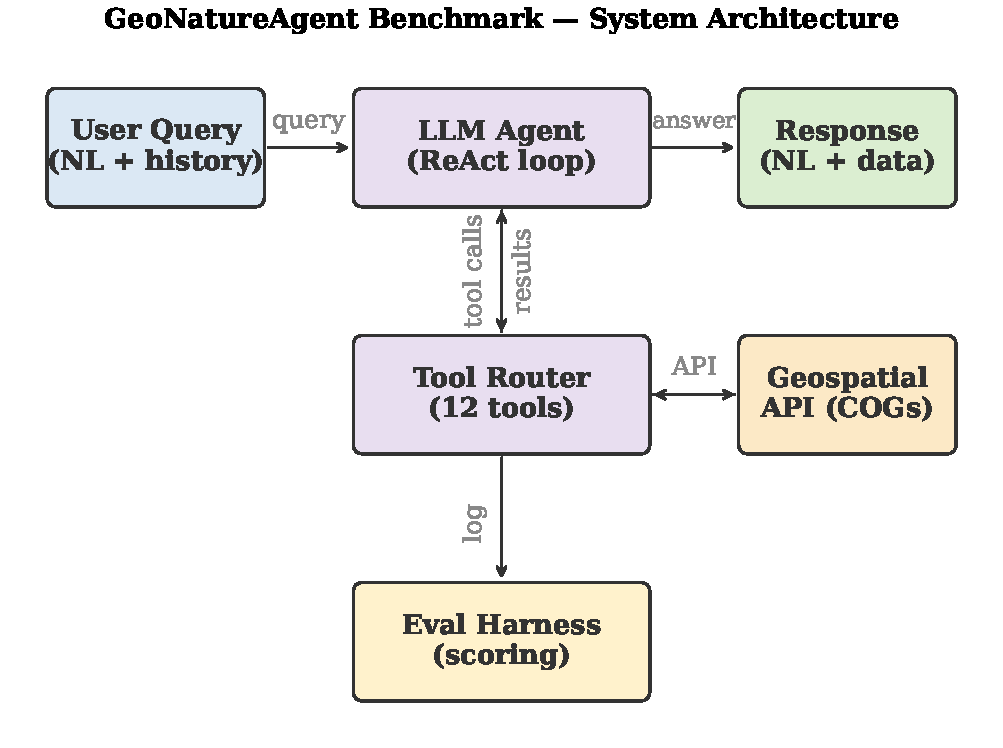
\includegraphics[width=\columnwidth]{figures/fig6_architecture.pdf}
  \caption{GeoNatureAgent Benchmark system architecture. The LLM agent interacts with a production API serving COG data; the eval harness logs all tool calls and scores responses.}
  \label{fig:architecture}
\end{figure}

\begin{table}[t]
\caption{Agent tools. The first eight are domain-specific; the last four are adapted from GeoBenchX~\cite{krechetova2025geobenchx}.}
\label{tab:tools}
\centering
\small
\begin{tabular}{ll}
\toprule
\textbf{Tool} & \textbf{Purpose} \\
\midrule
\texttt{lookup\_province} & Resolve province $\to$ boundary geometry \\
\texttt{lookup\_municipality} & Resolve municipality (+ province hint) \\
\texttt{analyze\_area} & Zonal statistics for indicator in AOI \\
\texttt{analyze\_multi\_layer} & Multi-indicator analysis in single call \\
\texttt{compare\_areas} & Compare two areas on same indicator \\
\texttt{find\_top\_n} & Rank provinces by indicator value \\
\texttt{toggle\_layer} & Enable/disable map layer visibility \\
\texttt{generate\_chart} & Bar/stacked-bar chart from data \\
\midrule
\texttt{create\_buffer} & Buffer geometry by distance (km) \\
\texttt{select\_spatial\_rel} & Select features by spatial predicate \\
\texttt{get\_centroids} & Extract centroid coordinates \\
\texttt{reject\_task} & Decline unsolvable tasks \\
\bottomrule
\end{tabular}
\end{table}

The design choice of structured tool calling over code generation is motivated by empirical evidence: GeoJSON~Agents report 85--97\% accuracy with function calling~\cite{luo2025geojsonagents}, while UnivEARTH reports only 33\% when agents generate executable code~\cite{kao2025univearth}.

\paragraph{Multi-backend inference client.}
Fair cross-model comparison requires normalizing heterogeneous API surfaces into a common interface. Our inference client routes models through two backends: a native Anthropic client for Claude, and a LiteLLM-based client for Vertex AI Model-as-a-Service (MaaS) endpoints that expose an OpenAI-compatible API. The MaaS backend maps publisher-prefixed model identifiers (e.g., \texttt{meta/llama4-...}) to Vertex AI endpoints and normalizes response formats---including tool-call representations---into the shared schema consumed by the eval harness. Notably, Llama~4 models emit tool calls as Python-style function invocations (\texttt{<|python\_start|>func(k=v)<|python\_end|>}) rather than JSON; a dedicated AST-based parser extracts these into structured tool calls, enabling Scout to achieve 5.4\% accuracy that would otherwise register as 0\%. Unattended execution of 744 model--task pairs requires robust failure handling: each inference call uses a layered timeout architecture combining daemon-thread hard timeouts with exponential-backoff retry on rate-limit errors.

\subsection{Evaluation Protocol}
\label{sec:scoring}

Each task is scored by eight check types (Table~\ref{tab:checks} and Figure~\ref{fig:scoring}). A task \emph{passes} only when \textbf{all} applicable checks pass (strict binary). We additionally compute partial-credit metrics for finer-grained analysis.

\begin{table}[t]
\caption{Scoring checks. Each task specifies which checks apply; a task passes only when every applicable check passes.}
\label{tab:checks}
\centering
\small
\begin{tabular}{lp{4.8cm}}
\toprule
\textbf{Check} & \textbf{Pass condition} \\
\midrule
\texttt{expected\_tools} & Every expected tool was called (recall\,=\,1.0). Extra tools do not cause failure.\textsuperscript{a} \\
\texttt{expected\_actions} & Every expected UI action was generated (recall\,=\,1.0). \\
\texttt{must\_contain} & Each required keyword appears in the answer (case-insensitive substring). \\
\texttt{must\_not\_contain} & No forbidden keyword appears in the answer. \\
\texttt{numeric\_accuracy} & For each ground-truth entry, the label is found in the answer and the nearest percentage value is within tolerance.\textsuperscript{b} \\
\texttt{chart\_generated} & At least one chart URL was produced (only checked when \texttt{generate\_chart} is an expected tool). \\
\texttt{max\_rounds} & Agent loop iterations $\leq$ budget. \\
\texttt{max\_cost\_usd} & Estimated token cost $\leq$ budget. \\
\bottomrule
\end{tabular}
\vspace{2pt}
\raggedright\footnotesize
\textsuperscript{a}Tool F1 (precision, recall, F1 on unique tool sets) is computed as a continuous metric but is not used as a gate.
\textsuperscript{b}A 120-character window after the label is searched for the first \texttt{float\%} pattern; tolerance defaults to $\pm$2\,pp.
\end{table}

\textbf{Continuous metrics.} Beyond binary pass/fail, we report: \emph{check score}---fraction of individual checks passed per case (partial credit); \emph{keyword coverage}---fraction of \texttt{must\_contain} terms found; \emph{tool F1}---set-based F1 between expected and actual tools; and \emph{cost utilisation}---ratio of actual to budgeted cost.

\textbf{Error classification.} When a task fails, the first failing check (in priority order: tool\_missing $\to$ chart\_missing $\to$ wrong\_data $\to$ rounds\_exceeded $\to$ cost\_exceeded $\to$ keyword\_missing $\to$ forbidden\_keyword) determines the error category. This priority reflects diagnostic value: tool selection failures are the most informative for understanding agent reasoning.

\textbf{Design rationale.} Tool and action checks use \emph{recall} as the gate rather than F1. An agent that calls all expected tools plus an exploratory extra tool should not be penalised---the key question is whether it performed the required operations. F1 is tracked as a separate metric for efficiency analysis.

\begin{figure}[t]
  \centering
  
\includegraphics[width=\columnwidth]{figures/fig8_scoring_pipeline.pdf}
  \caption{Scoring pipeline. Each case is evaluated by up to eight checks; binary pass requires all to pass. Partial-credit metrics (check score, tool F1, keyword coverage) are always computed.}
  \label{fig:scoring}
\end{figure}

\subsection{MLOps Pipeline}

Experiments are defined as YAML configuration files. A Cloud Build pipeline builds a Docker image, deploys a Cloud Run Job executing all experiments sequentially, and generates structured outputs: \texttt{results.jsonl} (per-case with full answer, conversation traces, tool inputs/outputs), \texttt{\_run\_meta.json} (frozen config + environment), and a batch-level \texttt{\_batch\_summary.json} with leaderboard, per-experiment metrics, and per-case Q\&A. All results are grouped under a run-level GCS prefix for isolation and traceability.


%% ══════════════════════════════════════════════════════════════════════════
\section{Experiments and Results}
\label{sec:results}

\subsection{Experimental Setup}

We evaluate eight LLMs on GeoNatureAgent Benchmark v5 (93 tasks, 18 categories) across Vertex~AI Model-as-a-Service and the Anthropic native API (Table~\ref{tab:models}). All experiments use the v3 system prompt (zero-shot), \texttt{max\_turns=10}, \texttt{max\_tokens=4096}, and \texttt{temperature=1.0}. Experiments run sequentially inside a single Cloud Run Job to ensure identical infrastructure conditions.

\begin{table}[t]
\caption{Models evaluated. Seven via Vertex AI; Claude via native Anthropic API.}
\label{tab:models}
\centering
\small
\begin{tabular}{llrl}
\toprule
\textbf{Model} & \textbf{Provider} & \textbf{Params} & \textbf{Access} \\
\midrule
GLM-5 & Zhipu AI & --- & Vertex MaaS \\
DeepSeek V3.2 & DeepSeek AI & 671B MoE & Vertex MaaS \\
Qwen3-235B & Alibaba & 235B MoE & Vertex MaaS \\
GPT-OSS-120B & OpenAI & 120B & Vertex MaaS \\
Gemini 2.5 Pro & Google & --- & Vertex native \\
Llama 4 Scout & Meta & 109B MoE & Vertex MaaS \\
Llama 4 Maverick & Meta & 400B MoE & Vertex MaaS \\
Claude Sonnet 4 & Anthropic & --- & Anthropic API \\
\bottomrule
\end{tabular}
\end{table}


\subsection{Overall Results}

\begin{figure}[t]
  \centering
  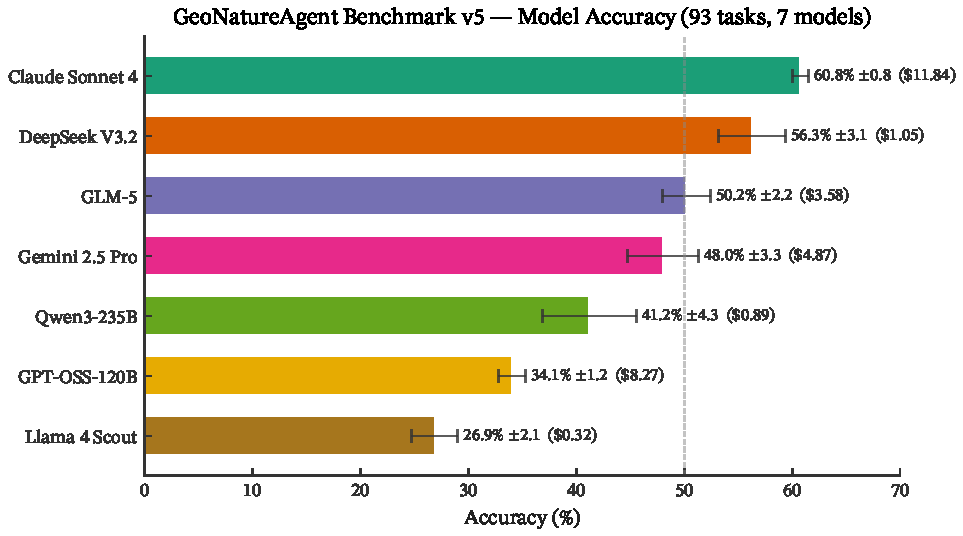
\includegraphics[width=\columnwidth]{figures/fig1_leaderboard.pdf}
  \caption{GeoNatureAgent Benchmark v5 leaderboard. Accuracy (\%) with total cost in parentheses. Dashed line at 50\%.}

  \label{fig:leaderboard}
\end{figure}

Table~\ref{tab:leaderboard} and Figure~\ref{fig:leaderboard} present the main results. GLM-5 and Claude~Sonnet~4 share the top position at 58.1\%, followed by DeepSeek~V3.2 (52.7\%) and Qwen3-235B (47.3\%). Three models exceed 50\%, yet no model surpasses 60\%, confirming that environmental geospatial tool orchestration remains a significant challenge even for frontier models. The top five models cluster between 40--58\%, with a sharp drop to Llama~4~Scout (5.4\%). Llama~4~Maverick returned 0\% due to persistent Vertex~AI infrastructure errors (HTTP~500) across all 93 cases; we report this as an availability finding rather than a model capability result.

Claude~Sonnet~4---the only model accessed via a native provider API rather than Vertex~AI MaaS---ties with GLM-5 for first place with notable strengths on municipality analysis, ranking, threshold tasks, and BigEarthNet land cover cases (83\% on the 24 BigEarthNet-related cases). However, it is the most expensive model at \$0.087/case, making it 3$\times$ costlier than GLM-5.

\begin{table}[t]
\caption{Leaderboard: 8 models on 93 GeoNatureAgent Benchmark v5 tasks. Cost is total for all 93 cases.}
\label{tab:leaderboard}
\centering
\small
\begin{tabular}{rlrrr}
\toprule
\textbf{\#} & \textbf{Model} & \textbf{Acc.} & \textbf{Cost} & \textbf{\$/case} \\
\midrule
1 & GLM-5            & 58.1\% & \$2.54  & .027 \\
1 & Claude Sonnet 4  & 58.1\% & \$8.13  & .087 \\
3 & DeepSeek V3.2    & 52.7\% & \$0.79  & .008 \\
4 & Qwen3-235B       & 47.3\% & \$0.50  & .005 \\
5 & Gemini 2.5 Pro   & 39.8\% & \$2.99  & .032 \\
5 & GPT-OSS-120B     & 39.8\% & \$4.77  & .051 \\
7 & Llama 4 Scout    &  5.4\% & \$0.04  & .000 \\
8 & Llama 4 Maverick &  0.0\% & ---     & --- \\
\bottomrule
\end{tabular}
\end{table}

\textbf{Partial credit tells a different story.} Even failing cases often demonstrate partial competence: correct tool selection but missing a keyword, or correct keywords but an extra unnecessary tool call. This gap between binary accuracy and partial-credit scores (Figure~\ref{fig:binary_partial}) suggests that many failures are ``near-misses'' addressable through prompt engineering.

\begin{figure}[t]
  \centering
  
\includegraphics[width=\columnwidth]{figures/fig3_binary_vs_partial.pdf}
  \caption{Binary accuracy vs partial-credit check score. The gap indicates many ``near-miss'' failures.}

  \label{fig:binary_partial}
\end{figure}


\subsection{Cost-Accuracy Analysis}

\begin{figure}[t]
  \centering
  
\includegraphics[width=\columnwidth]{figures/fig2_cost_accuracy.pdf}
  \caption{Cost-accuracy trade-off. Bubble size proportional to total tokens. Qwen3-235B and DeepSeek~V3.2 dominate the Pareto frontier.}

  \label{fig:cost_accuracy}
\end{figure}

Cost varies by an order of magnitude (Figure~\ref{fig:cost_accuracy}). Qwen3-235B offers the best cost-efficiency at \$0.005/case with 47.3\% accuracy, while Claude~Sonnet~4 costs 17$\times$ more (\$0.087/case) for the joint-highest accuracy (58.1\%). GLM-5 matches Claude's accuracy (58.1\%) at a moderate \$0.027/case. The Pareto frontier is dominated by Qwen3 (cheapest competitive option), DeepSeek (best accuracy-to-cost ratio at 52.7\%), and GLM-5 (highest accuracy at lowest cost among top models).

\begin{table}[t]
\caption{Projected daily cost at 1,000 queries/day.}
\label{tab:cost_projection}
\centering
\small
\begin{tabular}{lrrr}
\toprule
\textbf{Model} & \textbf{Accuracy} & \textbf{Daily Cost} & \textbf{Monthly Cost} \\
\midrule
Qwen3-235B      & 47.3\% & \$5   & \$150 \\
DeepSeek V3.2   & 52.7\% & \$8   & \$240 \\
GLM-5           & 58.1\% & \$27  & \$810 \\
Gemini 2.5 Pro  & 39.8\% & \$32  & \$960 \\
GPT-OSS-120B    & 39.8\% & \$51  & \$1,530 \\
Claude Sonnet 4 & 58.1\% & \$87  & \$2,610 \\
\bottomrule
\end{tabular}
\end{table}

Table~\ref{tab:cost_projection} shows projected costs for a production deployment. A service processing 1,000 queries/day would pay \$5--8/day with Qwen3 or DeepSeek (47--53\% accuracy) vs \$87/day with Claude Sonnet~4 for the highest accuracy (58.1\%)---a compelling case for empirical benchmarking over provider reputation. This finding echoes Geo-OLM's demonstration~\cite{stamoulis2025geoolm} that cost-efficient models can match frontier performance at dramatically lower cost.

Figure~\ref{fig:tokens_accuracy} further illustrates this relationship, showing that token consumption does not predict accuracy---models that generate more tokens do not necessarily achieve higher scores.

\begin{figure}[t]
  \centering
  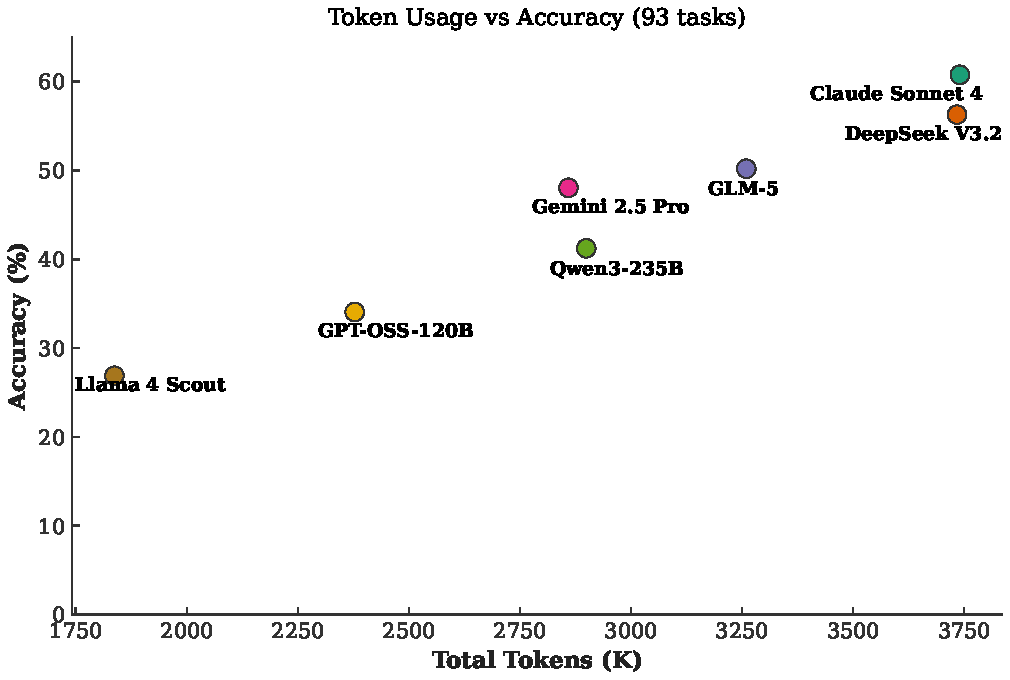
\includegraphics[width=\columnwidth]{figures/fig7_tokens_accuracy.pdf}
  \caption{Token consumption vs accuracy. Token volume is a poor predictor of performance.}

  \label{fig:tokens_accuracy}
\end{figure}


\subsection{Failure Analysis}

\subsubsection{Universally Hard Tasks}

One category achieved 0\% accuracy across all completed models (Figure~\ref{fig:hard_cases}), revealing a systematic limitation:

\begin{figure}[t]
  \centering
  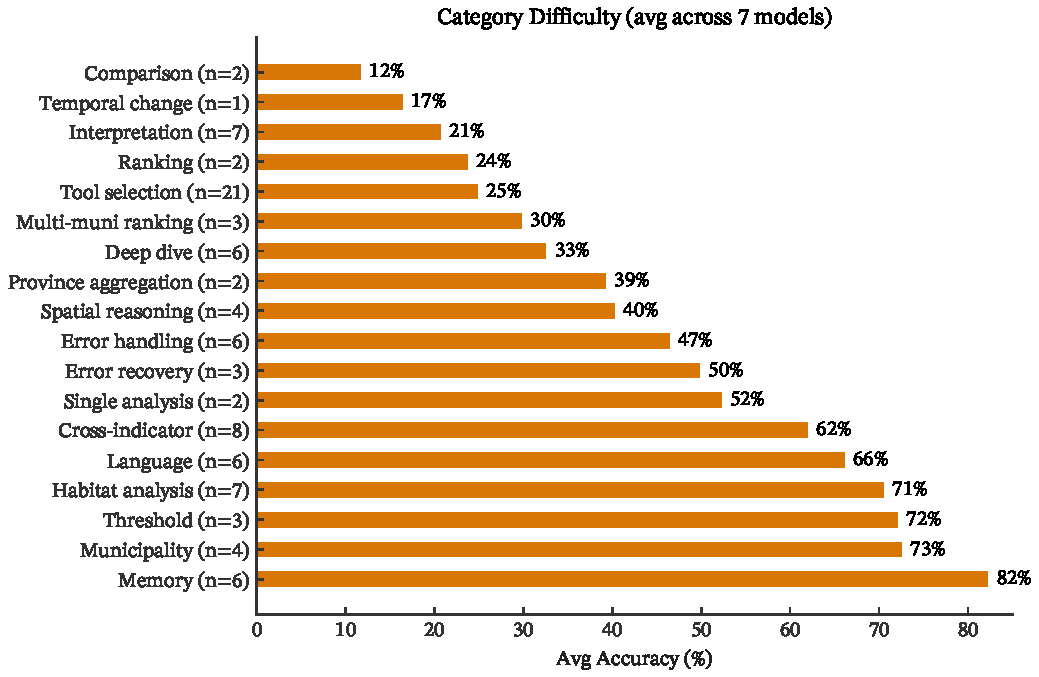
\includegraphics[width=\columnwidth]{figures/fig5_hard_cases.pdf}
  \caption{Universally hard categories---average accuracy across all completed models.}

  \label{fig:hard_cases}
\end{figure}

\textbf{Comparison} (0/2 for all models): close-value comparisons (e.g., Murcia 68.5\% vs C\'{o}rdoba 68.4\%) caused all models to fabricate differences rather than reporting near-identical values. \textbf{Deep dive} (0--50\%): multi-tool environmental profiling requiring sequential tool calls proved difficult, with most models solving at most two of six tasks. \textbf{Error recovery} (0--33\%): graceful fallback when data is unavailable was solved inconsistently across models.

Conversely, \textbf{error handling} was the easiest category: Qwen3-235B achieved 100\% (6/6), and GLM-5, Gemini, and GPT-OSS each scored 67\%. Models can recognise invalid inputs but struggle with multi-step analytical reasoning.

\subsubsection{Model-Specific Patterns}

\textbf{GLM-5} (58.1\%): co-leader, strongest on tool selection and the only model besides Claude to achieve high scores on ranking and province aggregation. \textbf{Claude Sonnet 4} (58.1\%): co-leader, strong on municipality analysis, ranking, threshold tasks, and BigEarthNet cases (83\% on the 24 BigEarthNet-related cases, highest among all models). However, it is the most expensive at \$0.087/case. \textbf{DeepSeek V3.2} (52.7\%): balanced across categories with particular strength in spatial reasoning, memory/multi-turn, and municipality analysis. \textbf{Qwen3-235B} (47.3\%): strongest on error handling, single analysis, and habitat analysis, but weakest on tool selection---correctly reasoning about \emph{what} to do but failing to invoke the right tool. \textbf{Gemini 2.5 Pro} (39.8\%): generated plausible-sounding answers from training data \emph{without calling any tools} in many cases---a hallucination pattern where the model bypasses the tool-calling protocol entirely. \textbf{GPT-OSS-120B} (39.8\%): moderate performance across categories with no standout strengths. \textbf{Llama 4 Scout} (5.4\%): only succeeded on a handful of cases (municipality and memory), failing all other categories; consistent with Vertex MaaS infrastructure instability for Meta models.


\subsection{Category-Level Analysis}

\begin{figure}[t]
  \centering
  
\includegraphics[width=\columnwidth]{figures/fig4_category_heatmap.pdf}
  \caption{Accuracy by category for six completed models. Comparison achieves 0\% across all models; error handling is near-solved.}

  \label{fig:heatmap}
\end{figure}

Figure~\ref{fig:heatmap} shows accuracy by category across the six completed models. Three key findings emerge: (1)~\textbf{comparison is universally unsolved} (0\% across all models); (2)~\textbf{error handling is near-solved} (17--100\%, with Qwen3 achieving 100\%); (3)~\textbf{language support is consistently strong} for the top six models on Galician and Basque inputs. The 21-case tool selection category---the largest---shows high variance across models, revealing that correct tool identification is model-dependent rather than category-dependent.


%% ══════════════════════════════════════════════════════════════════════════
\section{Discussion}
\label{sec:discussion}

\subsection{Comparison with Prior Benchmarks}

GeoNatureAgent Benchmark's 58.1\% best-model accuracy is notably lower than GeoBenchX and GeoJSON~Agents (85--97\%). Table~\ref{tab:benchmark_comparison} summarises the key differences.

\begin{table}[t]
\centering
\small
\caption{Comparison of structured tool-calling geospatial benchmarks.}
\label{tab:benchmark_comparison}
\begin{tabular}{lcc}
\toprule
& \textbf{GeoBenchX} & \textbf{GeoNatureAgent Benchmark} \\
\midrule
Tasks              & 202            & 93 \\
Categories         & 5              & 18 \\
Tools              & 24 primitives  & 12 domain ops \\
Tool abstraction   & Low-level      & High-level \\
Data source        & Local files    & Cloud API (COG + JSON) \\
Domain             & General GIS    & Environmental \\
Countries          & ---            & Spain + Portugal \\
Indicators         & ---            & 3 \\
Multi-turn         & No             & Yes \\
Best accuracy      & 85--90\%       & 58.1\% \\
Evaluation         & LLM-as-judge   & Metric-based \\
\bottomrule
\end{tabular}
\end{table}

Four factors explain the accuracy gap: (1)~real API interaction vs local file operations; (2)~environmental domain complexity (geographic knowledge, data limitations, display-only layers); (3)~multi-turn conversation history; (4)~strict binary evaluation. Our results align with harder benchmarks: MapEval ($<$67\%)~\cite{dihan2025mapeval}, SpatiaLab (55\%)~\cite{wasi2026spatialab}, UnivEARTH (33\%)~\cite{kao2025univearth}.

The GeoBenchX comparison is particularly instructive because both benchmarks share the structured tool-calling paradigm. The 27--39 percentage-point accuracy drop from general GIS tasks to environmental analysis suggests that general-purpose geospatial benchmarks substantially overestimate agent capability for domain-specific workflows. Environmental tasks require geographic knowledge (e.g., which provinces have erosion data), awareness of data limitations (display-only layers that cannot be analysed), multi-step reasoning across indicators, and temporal awareness---challenges absent from generic filter-merge-visualise pipelines. This motivates domain-specific benchmarks as a necessary complement to general-purpose evaluations.

\subsection{Structured Tool Calling vs Code Generation}

Our 58.1\% on real API tool calls compares favourably with UnivEARTH's 33\% on code generation~\cite{kao2025univearth}. While not directly comparable, the structured approach constrains the output space, eliminating the 58\% code execution failure rate. This provides further evidence that production environmental systems should prefer structured APIs over free-form code generation.

\subsection{Cross-Dataset Evaluation: BigEarthNet V2}
\label{sec:validation}

GeoNatureAgent Benchmark is designed to be domain- and geography-agnostic. To demonstrate extensibility beyond Spanish CO2 and erosion indicators, we incorporate BigEarthNet~V2~\cite{clasen2024reben} as a third data domain covering a different country. BigEarthNet~V2 provides 549k labeled Sentinel-2 patches with CLC2018 19-class labels; we aggregate the 75k+ Portuguese patches across 9 mainland districts into a 7-class land cover distribution (Coniferous Forest, Broadleaf Forest, Shrubland, Grassland, Sparse Vegetation, Water, Urban) queryable via the same \texttt{analyze\_area} tool used for Spanish indicators.

This integration tests whether agents generalise from Spanish environmental data to a different country and data domain. The 20 BigEarthNet benchmark cases (Table~\ref{tab:bigearth_cases}) span seven task patterns: single-district breakdown, cross-indicator synthesis (Portuguese land cover with Spanish CO2/erosion), multi-turn recall, chart generation, legend and layer discovery, temporal context, and two-district comparison. Unlike the CO2 and erosion indicators where ground truth depends on live raster geometry, BigEarthNet cases have fixed numeric ground truth derived from pre-computed district-level statistics, enabling deterministic scoring.

\begin{table}[t]
\caption{BigEarthNet V2 benchmark cases by task pattern. All cases use Portuguese districts with pre-computed ground truth.}
\label{tab:bigearth_cases}
\centering
\small
\begin{tabular}{lr}
\toprule
\textbf{Task Pattern} & \textbf{Cases} \\
\midrule
Single-district land cover breakdown     & 3 \\
Cross-indicator (PT land cover + ES)     & 3 \\
Multi-turn recall from session history   & 2 \\
Chart generation                         & 2 \\
Legend / list layers discovery            & 2 \\
Deep-dive multi-indicator profile        & 4 \\
Two-district comparison                  & 4 \\
\bottomrule
\end{tabular}
\end{table}

While Table~\ref{tab:bigearth_cases} lists the 20 purpose-built BigEarthNet cases, Portuguese land cover data also appears in 4 additional cases across other categories (tool selection, interpretation, error recovery), yielding 24 BigEarthNet-related cases in total. Across all 24, Claude~Sonnet~4 achieves the highest accuracy (83.3\%), followed by GLM-5 (58.3\%), and DeepSeek~V3.2, Qwen3-235B, and Gemini~2.5~Pro (all 54.2\%), with GPT-OSS-120B at 33.3\%. Claude's dominance on the BigEarthNet cases---despite sharing overall first place with GLM-5 at 58.1\%---suggests that its native API integration and stronger instruction-following enable more reliable handling of the Portuguese district lookup and JSON-backed indicator workflow. The three models tied at 54.2\% demonstrate consistent cross-country generalisation, while the gap to GPT-OSS-120B (33.3\%) highlights model-specific weaknesses in multi-step tool orchestration.

The inclusion of BigEarthNet~V2 as a queryable layer rather than merely a validation dataset transforms the benchmark's geographic scope from Spain-only to cross-country (Spain + Portugal), and its indicator count from two to three. This validates the claim that the framework generalises to new data sources: adding a new indicator required only a JSON statistics file, a prompt update, and new benchmark cases---no changes to the scoring engine or evaluation protocol.

\subsection{Limitations}

\textbf{Geographic scope}: benchmark tasks target Spanish provinces/municipalities and Portuguese districts, covering the Iberian Peninsula but not yet extending to other regions. \textbf{Indicators}: three analyzable layers (CO2 suitability, gully erosion, BigEarthNet~V2 land cover), though 18 task categories provide broad behavioural coverage. \textbf{Infrastructure availability}: Llama~4~Maverick returned persistent HTTP~500 errors from Vertex~AI across all 93 cases, yielding 0\% accuracy that reflects infrastructure failure rather than model capability. \textbf{Single-run}: temperature~1.0 introduces variance; no multi-run confidence intervals. \textbf{No prompt ablation}: all models use v3 zero-shot. \textbf{Evaluation strictness}: binary pass/fail may understate capability (Section~\ref{sec:scoring} describes the partial-credit metrics that address this).


%% ══════════════════════════════════════════════════════════════════════════
\section{Conclusion}
\label{sec:conclusion}

We introduce GeoNatureAgent Benchmark, a benchmark for evaluating AI agents on environmental geospatial analysis through structured tool calling against a production API. The benchmark spans three indicators across Spain and Portugal, demonstrating domain and geographic extensibility. Evaluating eight LLMs on 93 tasks across 18 categories with twelve tools:

\begin{enumerate}
  \item \textbf{Environmental geospatial tool orchestration remains open.} The best models (GLM-5 and Claude~Sonnet~4) achieve 58.1\%---well below the 85--97\% on general GIS benchmarks, with only three models exceeding 50\%.
  \item \textbf{Cost-accuracy trade-offs are dramatic.} DeepSeek~V3.2 achieves 52.7\% at \$0.008/case; Claude~Sonnet~4 costs 11$\times$ more for the highest accuracy (58.1\%).
  \item \textbf{Systematic failures persist.} No model passes comparison tasks; deep-dive profiling averages 30\% across models.
  \item \textbf{Real API interaction is more discriminative} than synthetic benchmarks, with a 27--32 percentage-point gap versus general GIS evaluations.
\end{enumerate}

\noindent\textbf{Future work}: expanding to additional countries and indicators (NDVI, precipitation, biodiversity indices); prompt ablation (zero-shot, CoT, few-shot); multi-run evaluation with confidence intervals; multi-agent architecture comparison following the Planner-Worker paradigm of GeoJSON~Agents~\cite{luo2025geojsonagents}.

GeoNatureAgent Benchmark, evaluation code, and the full MLOps pipeline are publicly available.\footnote{\url{https://github.com/darwin-geo/GeoNatureAgent}}


%% ══════════════════════════════════════════════════════════════════════════
\section*{Acknowledgments}

The authors thank Darwins Geospatial S.L.\ for providing the production API infrastructure used in this evaluation.

\bibliographystyle{plainnat}
\bibliography{references}

\end{document}
